\section{Introduction}\label{sec:introduction}

Nowadays, the protection of personal data has become a fundamental requirement of security. According to Tipton~\cite{Tipton:CRC:2003}, information security is concerned with the development of methods and tools for protecting information and preserving the value it has for an individual or an organization. For an efficient and effective protection, the use of robust authentication mechanisms is paramount.

Knowledge-based methods (e.g., password, secret question) and token-based methods (e.g., smart cards, token code) are probably the most used authentication mechanisms to date. However, both methods have a critical feature: at the time of authentication, the system does not verify who is requesting access, but rather what the users know or possess. This renders the system vulnerable, since that knowledge or an object can easily be lost, shared or manipulated. As an alternative, biometrics is an authentication mechanism considered more natural and reliable as it focuses on verifying who is the person requesting the access~\cite{Jain:IB:2011}. Biometrics provides methods for recognizing humans automatically based on behavior, physical or chemical traits, being fingerprint, face, iris, hand geometry, hand vein, voice and DNA, the most common traits used~\cite{Jain:IB:2011}.

Although there are several traits that can be used to perform user authentication, researchers are constantly looking for biometric traits with low acquisition and storage costs, that are less invasive, present a high degree of uniqueness and are stable. However, the static nature of a stable biometric trait suggests ``the paradox of secure biometrics''~\cite{Gorman:PIEEE:2003}:

\begin{quote}
\textit{``An authenticator must be stable and distinctive to be considered a good authenticator. But, stability leaves no option for compromise recovery, since users cannot change their biometric trait if stolen. Moreover, since a biometric clue is not secret, its information can be learned and copied.''}
\end{quote}

\vspace{0.3cm}

Although a stable biometric trait is an ideal authenticator, in practice, its use would not work if it were learned or copied. Therefore, researchers have striven to develop methods that detect whether a biometric sample presented to the acquisition sensor is a replica of the original sample. In the literature, the action of presenting a synthetic biometric sample of some valid user to the acquisition sensor in order to authenticate itself as a legitimate user is known as spoofing attack.

\minor{Among several forms of biometric, face recognition is of paramount importance with outstanding solutions presented thus far such as deformable models~\cite{Wiskott:TPAMI:1997}, texture-based representations~\cite{Ahonen:ECCV:2004}, and shape-based representations~\cite{Liu:TIP:2001}. Although effective in many cases, according to Maltoni et al.~\cite{Maltoni:HFR:2009}, face, signature and voice are the easiest biometric signals to be circumvented. For instance, spoofing attacks can be successfully accomplished in a face biometric system if an impostor obtains access by presenting to the acquisition sensor a photography, digital video or a 3D model of the target person~\cite{Jain:IB:2011}. Even with recent advances in biometrics, information forensics and security, the vulnerability of facial biometric systems against spoofing attacks is still an open problem.}

\minor{During the production of the synthetic biometric data, inevitably, there are noise information and telltales added to the biometric signal that can be captured and further processed to pinpoint attacks. In fact, in the manufacturing process of a synthetic sample, there are, at least, two re-quantization steps of the original biometric signal. In photo- and mask-based face spoofing attacks, the continuous signal is quantized during the digitization process. Then, this digital version is re-quantized due to the printing process with 2D and 3D printers and again digitized during the presentation of the synthetic data to the acquisition sensor. In video-based face spoofing attacks, the continuous signal is digitized and recaptured by the acquisition sensor during the attack.}
%
\begin{figure}[!htb]
\centering
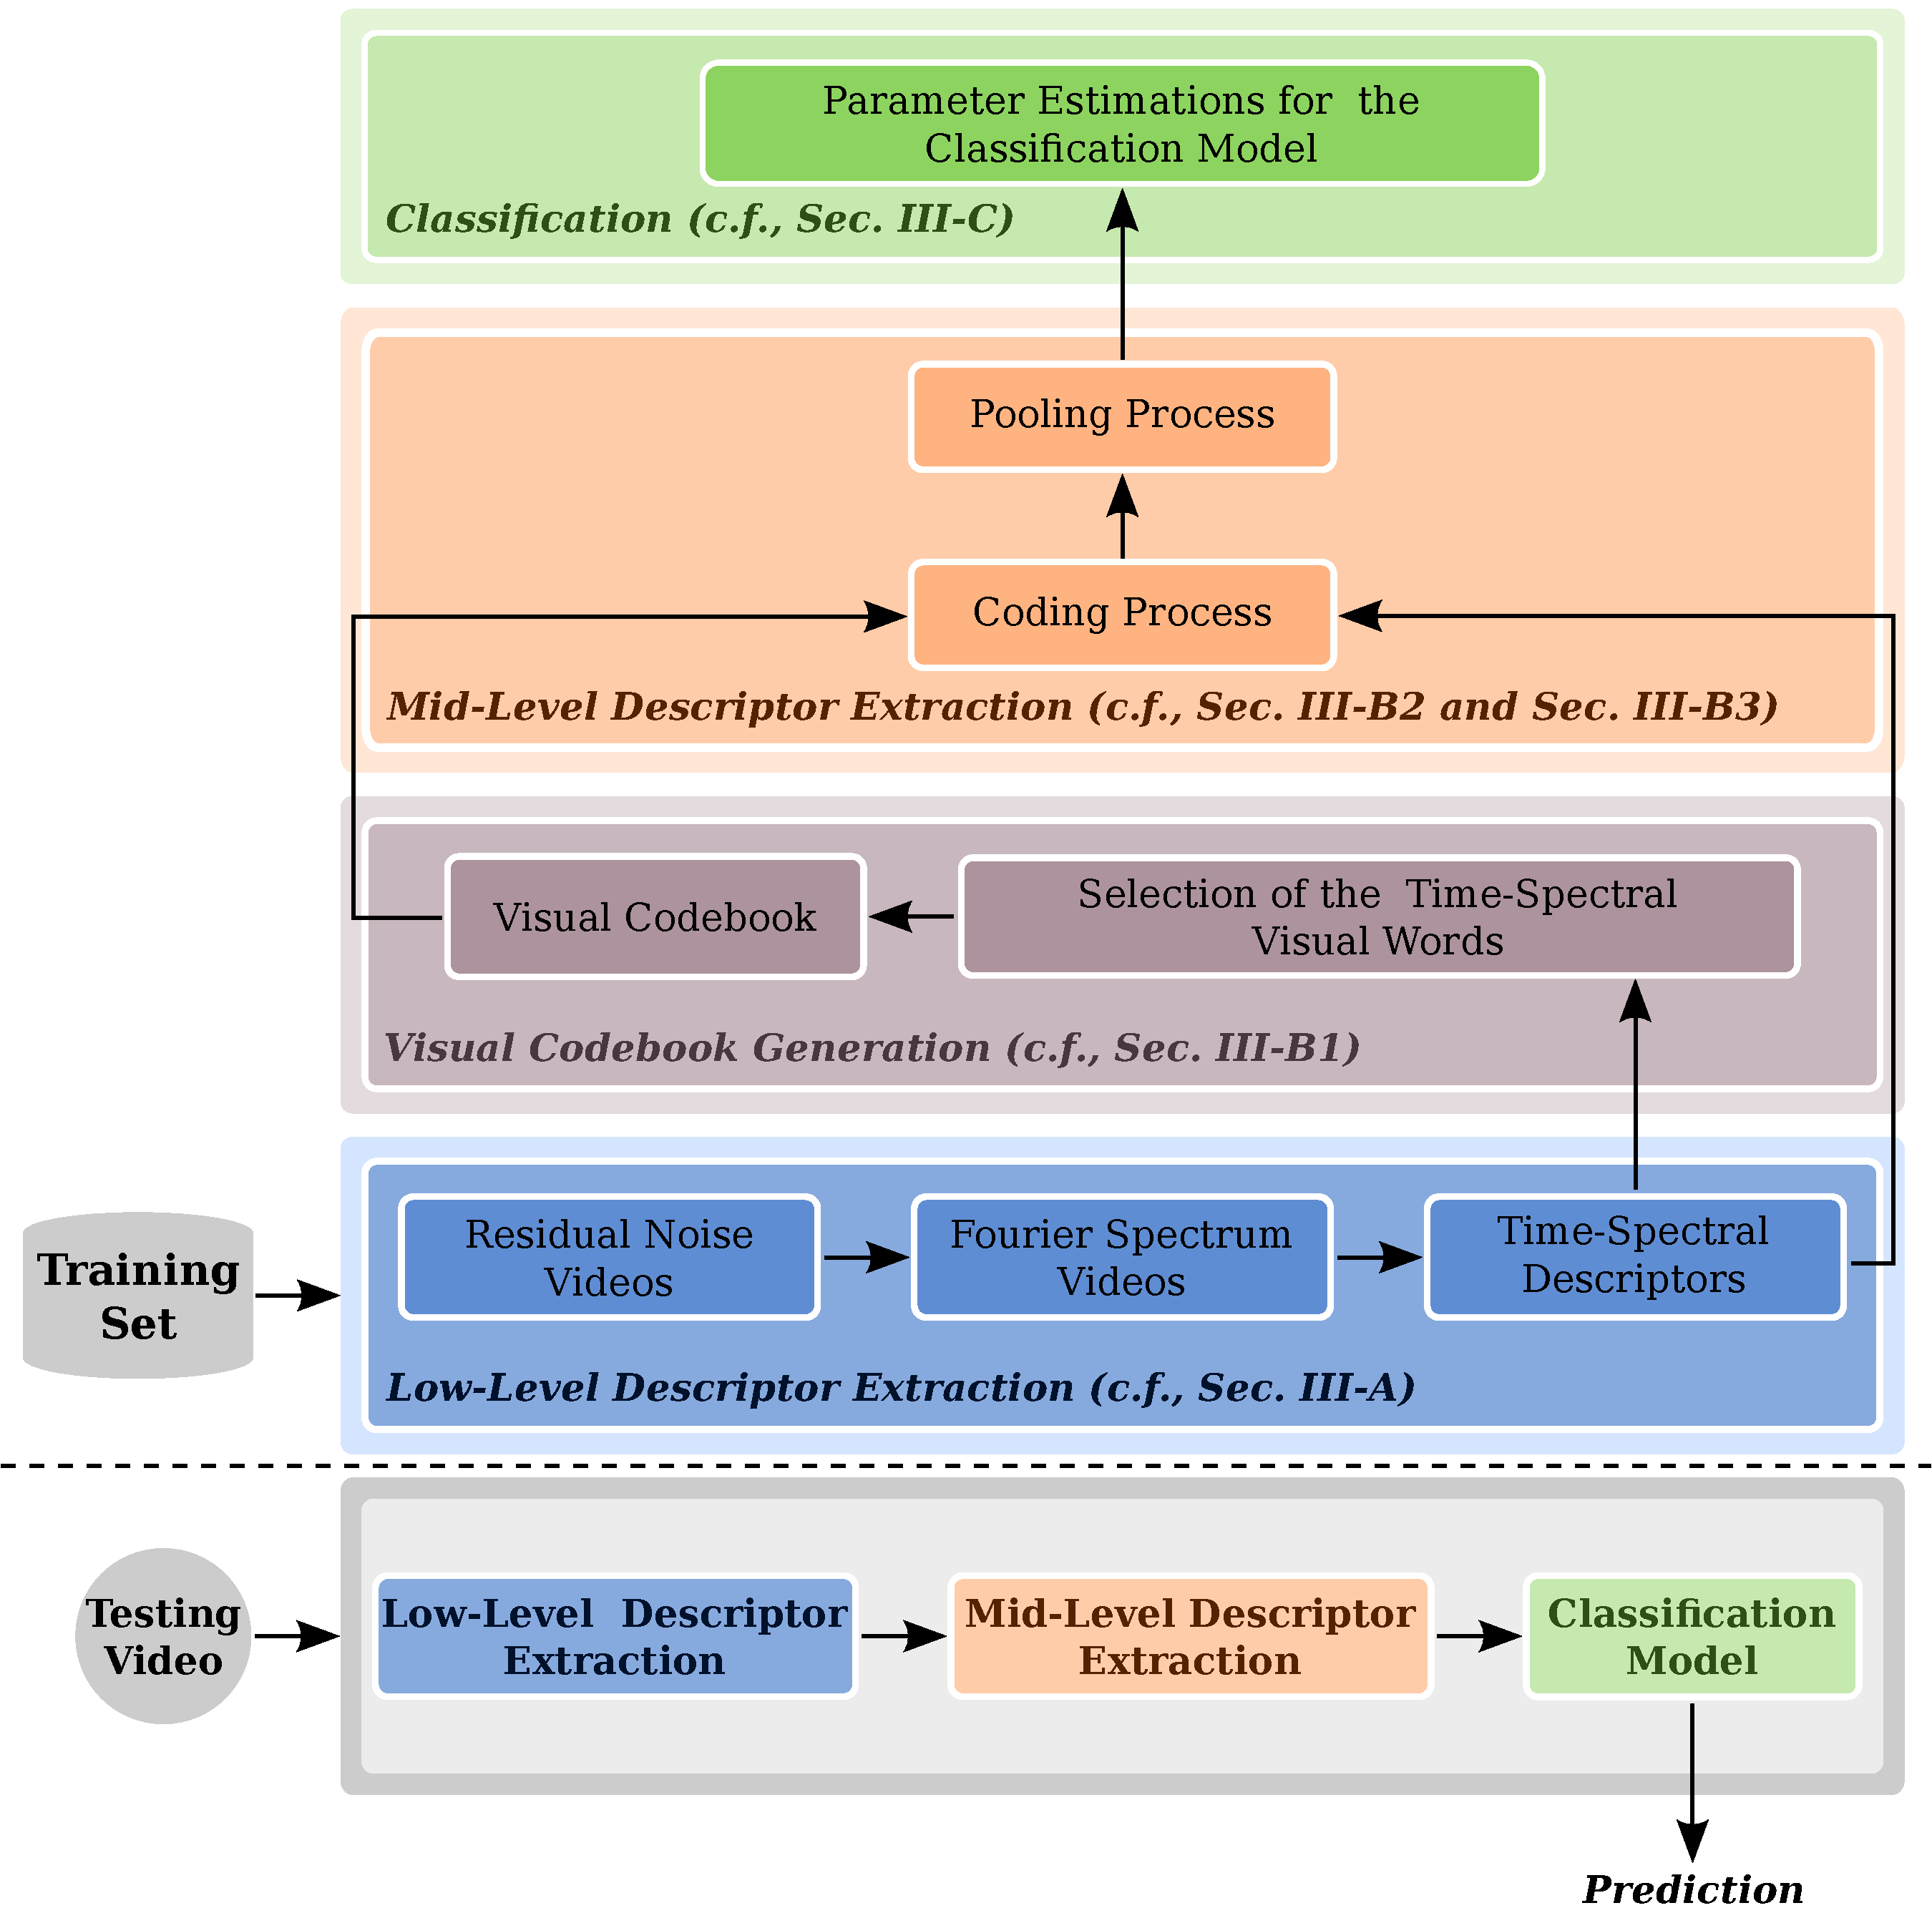
\includegraphics[width=0.45\textwidth]{method_overview_v1.pdf}
\caption{Main steps of the proposed method. Given a training set consisting of valid access and attempted attack videos, and also a testing video, we first extract a noise signature from every training video, generating a \allan{residual noise video}, and calculate its spectrum video. Then, we extract time-spectral descriptors from spectrum videos (low-level representation), which \minor{are used to generate} a visual codebook. With the visual codebook at hand, we transform the low-level descriptors in time-spectral visual word descriptors (mid-level representation). Finally, these mid-level descriptors are used to find parameters of the classification model, which \minor{are employed to predict} whether a given testing video is an attempted attack.}
\label{fig:method_overview}
\end{figure}

\minor{Recent works~\cite{Maatta:IJCB:2011, Pinto:SIBGRAPI:2012, Tan:ECCV:2010} show that noise and artifacts such as blurring effects, printing artifacts, banding effects, and Moir\'{e} patterns are added to the synthetic biometric samples during their manufacture and recapture. In this paper, we propose a spatio-temporal algorithm that captures such effects along time to provide an effective discriminative signature for valid access and spoofing attempts. In summary, the main contributions of this paper are:}
%
\begin{itemize}
	\item a new method for extracting temporal and spectral information from face biometric samples, referred to as time-spectral descriptors;
	\item evaluation of the visual codebook model, also referred to as Bag-of-Visual-Word model, for creating a mid-level representation from time-spectral descriptors, referred to as time-spectral visual words; and
	\item a low-cost solution for spoofing detection, \minor{illustrated in Figure~\ref{fig:method_overview}}, that does not rely on the user interaction or on extra hardware (e.g., infrared, motion or depth sensors) to detect different types of synthetic samples or attacks (e.g., photos, videos and masks) and is amenable to be implemented in computational devices such as PCs, handheld, and embedded systems. 
\end{itemize}

We organize the remaining of this paper as follows. Section~\ref{sec:relatedwork} discusses state-of-the-art methods for face spoofing attack detection. Section~\ref{sec:method} presents our method for spoofing attack detection. Section~\ref{sec:experimentalresults} shows and discusses the experimental protocol and the obtained results. Finally, Section~\ref{sec:conclusions} concludes the paper and discusses possible future work.
